\documentclass{article}
\usepackage[utf8]{inputenc}

\usepackage{natbib}
\usepackage{graphicx}

\begin{document}
	
\begin{titlepage}
	\begin{center}
		\vspace*{1cm}
		\LARGE \textbf{Synthesising emotion-driven images}
		
		\vspace*{1cm}
		\Large Konrad Cybulski
		
		\vspace*{0.5cm}
		\large 27807460
		
		\vspace*{2cm}
		
		
		
\includegraphics[width=0.4\textwidth]{images/monash_emblem.jpg}
		
		\vspace*{2cm}
		\Large Literature Review - Semester 1, May 2019
		
		\vspace*{1cm}
		\Large Supervisor: Jon McCormack
		
		\vfill
		
		\large Faculty of Information Technology
		
		\large Monash University
		
		\large Australia
		
	\end{center}

\end{titlepage}

\pagebreak

\tableofcontents

\pagebreak

\section{Introduction}

For centuries artists have been extremely talented at creating pieces of artwork that convey a range of emotions to those who view them.
Extensive research has been conducted into how visual features affect humans emotionally and how these can be used to predict and detect the emotional content of images and text \citep{machajdik2010affective, zhao2014exploring}.
Due to the subjective and qualitative nature of human emotion, assigning a quantitative measure of emotion to an image is no easy task.
Furthermore the ability to computationally recognise the emotional content of an image has wide-ranging applications from classifying posts on social media, to the creation of images, text, and even physical spaces in an emotionally quantifiable way.

This research aims to investigate representations for quantitatively representing emotion and its effect on image emotion classification
Primarily focusing on comparing categorical (happy, sad, etc.) and continuous (valence-arousal-dominance) representations for emotion in the context of image classification, and extending the learnings of such a classifier in image synthesis.
Through the generative process, gain a better understanding of visual patterns learnt by such a classifier by maximising classification confidence through the use of conditional generative adversarial networks \citep{gauthier2014conditional}, and evolutionary techniques explored by \citep{nguyen2015deep}.

Methods for quantifiably representing emotion have been explored thoroughly in the domain of psychology, with continuous multi-dimensional models being used in lieu of a single emotional label.
The circumplex model of emotion introduced a two-dimensional space characterised by valence, and arousal; respectively representing positivity or negativity, and the level of excitement associated with it \citep{russell1980circumplex}.
Such a continuous model is not without flaw, failing to accurately capture more complex emotional states, often those that represent concurrent conflicting sides of a given axis \citep{larsen1992promises}.
The complexity of such a continuous representation of emotion has been investigated in depth and extended in various ways, including through the addition of a third dimension: dominance \citep{bradley1994measuring}; which is particularly of interest within social dynamics.

The domain of emotion classification has had a particular focus on facial expressions and text \citep{cambria2016affective, warriner2013norms}.
Image emotion classifiers have been explored \citep{kim2018building, machajdik2010affective, chen2015learning, chen2014deepsentibank} yet their use has been limited.
Humans are able to fluently recognise, label, and discuss the emotional affect of an image, yet computers currently lack this ability.
However ongoing research is still further enabling and advancing the computational classification of image affect, and understanding the underlying patterns associated with image emotion.

As with the use of deep neural network image classifiers such as ResNet, AlexNet, and Inception, the shapes and patterns learnt by such deep learning systems are difficult to extract.
Recent work has looked at the use of quality-diverse generative algorithms with such deep classifiers \citep{nguyen2015deep, nguyen2015innovation}.
The underlying patterns learned by the classifier can be surfaced by synthesising images that maximise various desirable features.
This method allowed the exploration of images to which the classifier assigns a given label such as \textit{school bus} or \textit{lighthouse}, enabling a deeper understanding of the visual characteristics inherent to each class.
This process however does not limit itself to the use of evolutionary algorithms for image synthesis, with other techniques including the use of generative adversarial networks \citep{GAN}.

\section{Aims and Scope}

The primary focus of the proposed research is to produce an image emotion classifier, and to further leverage it in the process of emotion-driven image synthesis.
The two core themes explored are image generation techniques, and processes for classifying and generating emotional content.
As a result this literature review aims to explore and understand the progression of knowledge in the fields of emotion representation and classification, computational image synthesis, and affective content synthesis.
All of which represent the multiple facets of the proposed body of research with which an investigation into the use of image emotion classifiers for emotion-driven image generation will be explored.


\section{Models of affect}

The field of emotion classification has surged in recent years given a popularity and rising interest in the use of facial recognition, gesture, voice, and body language for emotion recognition.
Other research has focused on exploring ways in which emotion can be recognised in images, text, and more abstract content.
Underlying the area of affect classification and recognition is the process of representing affect and emotion in both a meaningful, and accurate way.
This section will discuss representations in the context of computational classification, in addition to their psychological underpinnings.

\subsection{Affect in psychology}

\textit{Affect} is a psychological term used to describe the experience or feeling of emotion.
Affect is fundamentally different to both emotion and feeling.
Feeling represents the label used to denote the inner processes triggered by situation and context \citep{shouse2005feeling}.
The term emotion represents the label attached to the resulting display of a feeling, often attributed to actions such as facial gestures, variation in desires, and changes in brain activity \citep{sloman2001beyond}.
Affect however represents the underlying internal and external causal relationships that result in variations of feeling and emotion or otherwise \citep{russell2003core}.
Affect as such represents the greatly more abstract underlying processes that are linked most closely to valence: positivity or negativity; and arousal: states of excitement or lack thereof \citep{russell2003core}.

Given the abstract nature of affect, we often measure and describe it through introspection of emotion and feeling, or observing their outward displays and projections.
As a result, shallow representations of emotion become widely used models of affect due to their simplicity.
Shallow models generally involve the translation of outward displays of emotion such as facial expressions, gestures, and brain activation, to their corresponding labels of emotion: happy, sad, etc \citep{sloman2001beyond}.
Aiming to capture more complex and deeper representations of emotion, \citet{sloman2001beyond} introduces the interpretation of emotion as the composition of information processing architectures.
In the field of artificial intelligence, and computing as a whole, models of affect are lacking in their ability to describe complex and semantically rich interactions between actors in addition to the effect of their environment \citep{sloman2001beyond}.

It is important however to recognise the advantages of what are deemed to be \textit{shallow} models of affect.
Shallow models enable the definition of a broad landscape of affective descriptors despite their inability to effectively define their relationships \citep{sloman2001beyond}.
More nuanced states of affect such as depression and embarrassment however represent states that a shallow and broad model fails to capture \citep{gunes2011emotion}.
Despite this, the use of categorical emotional states and labels represents the majority of research at the intersection of computing and affect \citep{gunes2011emotion}.
More complex relationships between the processes involved with affect, feeling, and emotion are often represented as dichotomous dimensional models, such as the two-dimensional model of valence and arousal (discussed below) in which each dimension represents polar states of affect \citep{grandjean2008conscious}.


\subsection{Categorical}

The computational recognition of emotion has been explored in countless studies and projects, in both the context of image emotion recognition \citep{machajdik2010affective,zhao2014exploring,kim2018building} and facial emotion classification \citep{mollahosseini2016going}.
However a core component and key difference between a large number of such bodies of research is the method by which emotion is represented.
Two of the most common representations represent a discrete, and continuous approach.

Discrete emotion representations generally involve the categorisation of emotion to a series of labels.
Discrete approaches represent the method used in a large number of papers \citep{machajdik2010affective,ali2017emotional,wangarttalk,mohammad2018wikiart} however the number of emotion labels explored varies greatly.
An example of the size of emotion label subsets used in studies of image emotion classification using such a discrete model are 7 \citep{ali2017emotional}, 8 \citep{machajdik2010affective}, 11 \citep{wangarttalk}, and even 19 \citep{mohammad2018wikiart}.
Due to this lack of consistency in emotion classification targets, such studies often repeat similar data gathering and classifier training methods again for their own use.
Despite the consequences of inconsistency in the emotion labels chosen, due to the simplicity of discrete categorical emotion assignment, data gathering can be performed with ease compared to continuous methods of emotion representation.
In order to create large image datasets of labelled images can be completed with greater ease when the number of such labels is reduced.
However there remains difficulty in labelling images with respect to emotion given the inherent variation in the emotional affect of an image, or accurately determining the emotion expressed by a facial expression.

The categorical representation is the simplest method for emotion classification, due not only to the consequent ease with which data can be gathered, but due to the extensive research surrounding methods for computational classification of content.
Many techniques for prediction, both for regression and classification rely on sufficiently large datasets of labelled data.
It is often difficult to determine the label of a datapoint computationally, since this ability would imply that such a predictive model already exists.
As a result dataset creation often involves a manual process of labelling datapoints.

Research in psychology has understood the increased error associated with continuous measurement tasked performed by humans in comparison to categorical classification \citep{harnad2003categorical}.
With the human brain's attempt to sort perceived objects and situations into learned categories, it has been shown to warp continuous variables and scales to do so.
As a result there exists an increased human error associated with the absolute measurements of continuous, compared to categorical variables.
However such absolute error can be mitigated by introducing comparative measurements in combination with a standard ranking algorithm such as \citet{glickman2012example,glickman1995glicko}.
Furthermore the introduction of processes such as the self-assessment manikin \citep{lang1980behavioral} assist the assessment of emotional affect associated with the circumplex model of affect (valence, arousal, and dominance).


\subsection{Continuous dimensional}

The aforementioned difficulty associated with labelling images according to their respective emotional content is accentuated with the introduction of a dimensionally continuous representation of emotion.
While proposed representations vary, the most recognised basis for many continuous models is the circumplex model of emotion \citep{russell1980circumplex}.
The circumplex model of emotion introduced by \citet{russell1980circumplex} asserts that emotion can be measured in terms of two continuous variables: valence, and arousal.
Valence measures the positivity or negativity associated with an emotion; and arousal measures the excitement associated with it.
For example, the discrete emotion label of \textbf{happiness} could be represented in the continuous valence-arousal (VA) space with high-valence, medium-arousal; while the label \textbf{depressed} would translate to low-valence, low-arousal; and \textbf{relaxed} being medium-valence, low-arousal.
While this continuous dimensional model allows for greater continuity in measuring emotions, it is not without fault \citep{larsen1992promises}.
The primary limitations of such a model involve it's likelihood of misinterpretation particularly when considering the labels of each dimension.
This issue of misinterpretation was of particular interest as the circumplex model of emotional affect was being refined and compared to other models emotional assessment such 
One way in which the circumplex model of affect introduced by \citet{russell1980circumplex} has been extended to address its weaknesses is through the introduction of a third-dimension: Dominance, the amount of control associated with an emotion.
Despite its limitations, the circumplex model has been used extensively in the field of psychology \citep{bradley1994measuring,warriner2013norms}, and in computational emotion classification to a limited extent \citep{zhao2016predicting}.

While both models for the representation of emotion have trade-offs, both suffer from issues related to cross-cultural differences in emotion expression and recognition.
Cultures inherently differ with respect to how emotions are both felt and expressed \citep{markus1991culture}; this becomes increasingly evident when attempting to classify the affective emotion embodied and expressed by more abstract content such as imagery and sound.
The popular image-emotion dataset used for classification known as the International Affective Picture System (IAPS) was shown to have a significantly different valence-arousal assignment for up to 31.74\% of images between Chinese and American young adults \citep{huang2015affective}.
Even with respect to the distribution of image valence-arousal values as assigned within a group of the same culture, these values often vary.
This culture-independent variation can be reduced by introducing valence-arousal assignment guidelines and benchmark comparisons.
One of the most commonly used methods for emotional affect self-assessment is the self-assessment manikin (SAM) \citep{lang1980behavioral}.
SAM, as can be seen in Figure \ref{fig:SAM}, was developed to aid in the evaluation of emotion, particularly its translation into the commonly used three dimensions of the circumplex model of affect: valence, arousal, dominance.
It has proved itself as more accurate and effective than other methods of emotion self-assessment while being less complex \citep{bradley1994measuring}.

\begin{figure}[h!]
	\centering
	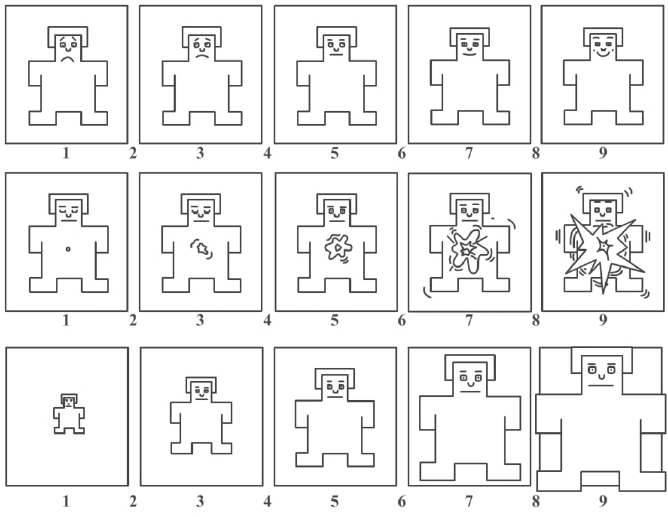
\includegraphics[width=0.75\textwidth]{images/self-assessment-manikin.png}
	\caption{The self-assessment manikin: a guide for reporting individual emotional affect in the three dimensions valence (top), arousal (middle), and dominance (bottom) as introduced by \citet{lang1980behavioral}}
	\label{fig:SAM}
\end{figure}

While both discrete and continuous methods of representing emotion have their respective benefits and trade-offs, the choice to use one over another often depends on the way in which the data gathering process for content emotion classification is performed.
These two representations of emotion can be translated between, since all categorical emotions can be converted to the continuous circumplex model, and the inverse.
However due to the higher complexity nature of the continuous model, even with the use of SAM, dimensional representations are more difficult to gather on a large scale in comparison to categorical emotions.


\section{Image classification}

Emotion classification has been researched in depth particularly with respect to two sub-domains: facial emotion recognition, and content emotion classification (image, text, sound).
Facial emotion recognition has been more heavily researched in this field when compared to content emotion classification.
While the applications of content emotion classifications seem to be few in comparison with those of facial recognition, the field has widely been explored in the context of text emotion classification, with image and sound emotion classification trailing behind.

Emotion classification has itself been a domain built upon the foundation of image classification techniques.
From hand-crafted feature decomposition, to neural network architectures, the emotional content of images and text rely heavily on findings in other domains such as image object classification and text sentiment analysis.

\subsection{Image object classification}

As the basis for many further computer vision applications, image object classification has been a primary focus of research in the field of machine learning.
The techniques associated with such tasks have for the most part in recent years involved the use of deep convolutional neural networks, which have proven to be state-of-the-art classifiers, with several high performing architectures such as ResNet, AlexNet, and Inception being used as staple image classifiers in other domains \citep{pan2009survey}.
While neural networks and their use date back to the 1980s, the higher availability and lower cost of single-instruction multiple-data (SIMD) processing architectures such as graphics processing units (GPU) has allowed for their widespread use \citep{rawat2017deep}.

Up until such time as neural network architectures could be fully leveraged, the majority of image classification tasks lent on manually deriving image features for use in other more traditional classification models (regression, support vector machines, etc.).
As a result the limiting factor of such classifiers were predictors derived from extracted image features.
The use of such extracted image features has its benefits however.
Their primary advantage lies particularly in relation to such features being more interpretable and human-understandable.
The features extracted from neural network classifiers however are often abstract and may lack any human-comprehensible parallels despite their comparative predictive advantage.
While it is often seen to be a black-box, the features learnt by a deep convolutional neural network, or any neural network architecture for that matter, do represent a repeatable and content-dependent image feature representation.
As such the ability to reuse such neural networks and their feature extraction capabilities has been thoroughly explored in various bodies of work \citep{kim2018building,pan2009survey,you2015robust}.
This practice is known as transfer learning.

\subsection{Neural networks} \label{sec:neural-network-overview}

This section will give a brief overview of neural networks and their application in image and content classification.
The principles underlying neural networks are simple, yet their ability to capture and learn highly complex non-linear representations of information has resulted in their popularity.
The fundamental building block of neural networks is the neuron, which itself is a parameterised mathematical function with which a range of inputs can be mapped to a single, or multiple outputs.
Examples of such mappings range from simple mathematical functions such linear or logistic regression, to more complex applications involving convolution and functions of input sequences.

Convolutional neural networks represent current state of the art when using images or text for classification or prediction.
First introduced by \citet{krizhevsky2012imagenet} as part of the ImageNet image classification competition, it exceeded the state-of-the-art at the time in classification accuracy.
The way in which such an architecture processes image input data is through convolutional layers.
As depicted in figure \ref{fig:CNN}, each neuron in a convolutional layer takes as input, a spatial subset of the layer before it.
The result is layers of neurons that have a greater deal of local spatial awareness when compared to the most commonly used fully connected layers.
The spatial constraints associated with these layers lends itself to the domain of image processing particularly given the highly spatial relationship of image pixels.

\begin{figure}[h!]
	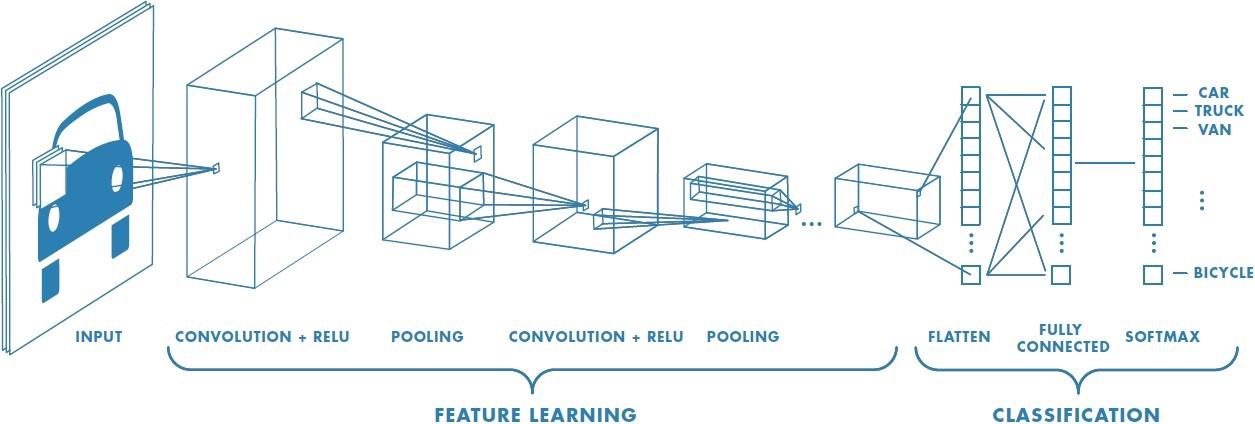
\includegraphics[width=\textwidth]{images/convolutional-neural-network.jpg}
	\caption{Visual representation of most convolutional neural network image object classifier structures as introduced by \citet{krizhevsky2012imagenet}}
	\label{fig:CNN}
\end{figure}

\subsection{Transfer learning}

Given the large amount of work conducted into image object classification, producing neural networks such as AlexNet, ResNet, and Inception, transfer learning has been heavily relied upon in various domains of classification and synthesis of images \citep{pan2009survey}.
Each of these commonly used object classification architectures have been originally trained on common baseline image object classification datasets such as CIFAR-10, CIFAR-100, and ImageNet.
These are three of the most common and widely-used image object classification datasets, in which images fall into one of 10, 100, and 1000 categories respectively.
As a result, the number of outputs of neural networks trained on these datasets is the total number of predictable categories.
Each of these pre-trained image classifiers can be used in other domains of machine learning by omitting the last layer of their architectures, which represent the object classification layer, and feed the previous feature layer into a new architecture.
In doing so, the information held within the neural network can be repurposed, and the learnings reused in other domains of application.

The use of transfer learning in numerous domains has increased the general ability to produce highly accurate networks even with comparatively small datasets.
Not only do the feature layer dimensions of each architecture differs, the features they represent vary.
As a result, using stacked predictor architectures, in which multiple feature vectors from multiple neural network classifiers are used as input to a further predictor network \citep{kim2018building}.
Using such a stacked predictor architecture enabled \citet{kim2018building} to generate a highly accurate image emotion classifier using a relatively small dataset of 10766 images.

The subjectivity and human-dependent nature of emotion has naturally resulted in only small datasets of emotion-labelled images.
Through transfer learning, pre-trained image object classifiers reduce the both the computational and dataset size requirements \citep{pan2009survey} for creating new predictive models.
Particularly in the domain of image emotion, transfer learning has enabled accurate classifiers to be built with relatively small image datasets (e.g. 10766 \citep{kim2018building}) by extracting the image features derived by image object classifiers such as ResNet and AlexNet.
Small datasets such as this however can benefit from other techniques such as data augmentation \citep{perez2017effectiveness} which through various image transformations such as rotation, cropping, blurring, and colour distortions, can increase the effective number of images available for training.
This technique, in combination with transfer learning is the foundation of research by \citet{wangarttalk} to create an art emotion and theme classifier.
Furthermore exploring simple variations on the transfer architecture, to determine the impact of a varying number of network layers taking as input, the feature vector of VGG and ResNet object classifiers.
This differs from the stacked feature extraction approach by \citet{kim2018building} with considerable success despite.

Transfer learning represents a core component of classifier architectures to leverage vast amounts of work done to train image object classifiers \citep{krizhevsky2012imagenet,pan2009survey} in domains that suffer from issues such as small datasets.
While opportunities exist to maximise accuracy through image classifier stacking for feature extraction \citep{kim2018building}, simpler architectures involving a single image object classifier and less than three hidden layers to process these features \citep{wangarttalk} have shown to provide considerably good results.


\subsection{Image emotion classification}

The area of image emotion and sentiment classification has been explored in a number of ways, primarily through image feature analysis derived from art and psychological factors \citep{machajdik2010affective}; and more recently using techniques such as deep neural networks \citep{chen2015learning, kim2018building}.
Feature extraction and analysis has been used for various applications such as measuring aesthetic appeal \citep{den2010using,den2010comparing,den2011evolving} and as an emotional feature vector for sentiment classification \citep{machajdik2010affective}.
Due to the artistic and psychological underpinnings used by \citet{machajdik2010affective}, the low-level features extracted from images can be understood at a high level.
The relationship between an image's emotion and its core artistic components such as balance, harmony, and variety was further explored by \citet{zhao2014exploring}, which uses a comparably small feature vector to \citet{machajdik2010affective}, resulting however in a 5\% classification increase to state-of-the-art approaches at the time.

Deep neural networks in this domain provide less transparency to the process with which emotions and sentiment are classified compared to feature analysis.
The emotional content of an image can be decomposed in various ways.
Image databases with singular emotion labels, and adjective-noun pairs (ANP) have been used for the training of deep neural network classifiers \citep{chen2014deepsentibank, yang2018visual} with up to 200\% performance gains over support vector machine classifiers.
The artificial neural network approach to general image classification domains has exploded in popularity when compared to feature decomposition approaches used by \citet{machajdik2010affective}.
This is largely due to their learning ability, particularly in recognising "hierarchical representations" \citep{lipton2015critical} of image features; which provides greatly improved performance when compared with manually crafted metrics derived through image decomposition.
This hands-off approach to image feature vector decomposition has further lent itself to techniques such as transfer learning.

The use of continuous emotion representations, particularly relating to the circumplex model have been explored in image emotion recognition tasks \citep{kim2018building, zhao2016predicting, zhao2017continuous}.
Regression models produced to predict the valence-arousal (VA) values of given images have shown high accuracy on various datasets.
In leveraging pre-trained image classification networks through transfer learning, even smaller datasets (10,000 images) can have high accuracy classification results \citep{kim2018building}.
Despite the aforementioned difficulty associated with labelling images on continuous dimensions such as the circumplex model of affect \citep{russell1980circumplex}, \citet{zhao2016predicting} have used image descriptions and comments to generate an image's respective valence, arousal, and dominance values.
\citet{zhao2016predicting} further use this dataset with hypergraph learning techniques for the personalised prediction of an image's emotional affect.
While categorical classification is more easily verified by humans, training predictive models with data that has an element of noise and uncertainty benefits from both continuity and volume.
This is a key advantage of the circumplex model as applied by \citet{kim2018building} and \citet{zhao2016predicting} in image emotion recognition over categorical classification.


\section{Computational image synthesis}

Computer-generated images (CGI), have been a widely used in the film industry, as well as in countless other domains such as gaming, simulation, and art.
CGI has, for the most part, involved human interaction, and human-controlled image and model generation.
While extensive research has been conducted into the generation of visually aesthetic images, applications of image synthesis extend to the synthesis of text to describe a given image \citep{mathews2016senticap}, as well as the generation of an image according to a target caption \citep{reed2016generative,zhang2017stackgan}.


\subsection{Evolutionary computing}

Some of the first methods for image generation focused on the synthesis of visually appealing images.
While often using human-in-the-loop systems, visually striking and aesthetic images were the goal of methods introduced by \citet{sims} and \citet{nevar} involving evolutionary techniques.
The \textit{NEvAr} \citep{nevar} system for the interactive evolution of images exemplifies the range of visual outputs possible with these techniques.
Evolutionary art leveraged methods introduced and exemplified by \citet{sims}, producing images such as those shown in Figure \ref{fig:sims}.
\citet{sims} proposed using \textit{Lisp} expressions for genotype definitions, which map a coordinate (x, y) into a grayscale or RGB value.
This genotype representation leveraged extensive research done into the use of evolutionary computing for optimisation problems.
This genotype expression has been used in numerous further research of both supervised and unsupervised image synthesis through evolutionary techniques \citep{nevar, sims, den2011evolving, distributed-evolutionary-art, aesthetic-measures}.
However the way in which NEvAr and Sims evolved images involved the manual process of selecting individuals in the population they deemed to be of higher fitness than the rest.

\begin{figure}[h!]
	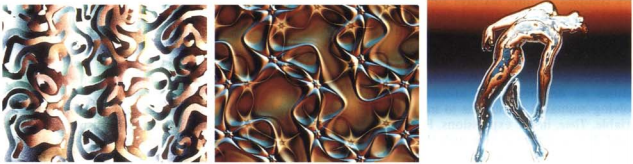
\includegraphics[width=\textwidth]{images/sims-interactive-image-generation.png}
	\caption{Images generated through the process of interactive evolution introduced by \citet{sims}}
	\label{fig:sims}
\end{figure}

Evolutionary computing techniques for image synthesis have been able to produce increasingly interesting and appealing imagery and artwork.
While the genotype representation introduced by \citet{sims} has formed a basis for further research in the field of evolutionary image synthesis \citep{den2011evolving,den2010using,nevar,den2012maintaining,distributed-evolutionary-art}, other genotype representations for image synthesis have been explored.
While common generative representations have involved the use of expression trees \citep{sims,nevar,aesthetic-measures}, methods such as direct pixel encodings \citep{nguyen2015deep}, and the more novel technique of line-drawing \citep{annunziato1998nagual,niche-reproduction}
Line-drawing as exemplified by \citet{niche-reproduction} has built upon evolutionary techniques, using a collection of individuals interacting in real-time to synthesise artwork.
In a traditional well-mixed \citep{sims} or distributed population \citep{distributed-evolutionary-art} each individual represents an image, or a model for generating one.
The particle swarm technique employed by \citet{niche-reproduction} however, generates images through the interaction of actors all of whom draw on the same canvas.
This real-time evolutionary image drawing mechanism, while producing visually interesting images, has not been explored with regard to its use in other application domains.


\subsection{Measures of aesthetics}

Despite the slow nature of the interactive process, \citet{sims} and \citet{nevar} were able to produce images with visually striking characteristics.
\citet{aesthetic-measures} investigated measures of aesthetics for fitness evaluation in artificially evolving images.
This research primarily used observations by \citet{ralph-bell-curve}, that the distribution of colour gradients in fine art tend toward normal.
While the images produced through this method did not meet the level of intricacy and detail as the results of \citet{sims} or \citet{nevar}, it represented a self-contained system able to generate appealing imagery without human interaction.

Measures of aesthetics have been explored and multiple have been derived using information about fine art \citep{ralph-bell-curve}, and others measuring levels of symmetry, and even complexity measures according to image compression ratios \citep{den2010using}.
Work by \citet{den2014investigating} performed a comparison of seven measures of aesthetics, comparing even some of the most popular metrics such as the Ralph bell curve \citep{ralph-bell-curve}.
The primary finding of this work showed that the visual styles and nature of the images depended heavily on the given aesthetic metric used to determine fitness.
Particularly given that the process by which images are generated is an optimisation problem, maximising the aesthetic value as measured by the given metric, the metric used has an immense impact on the resulting styles.
However it was found that various pairs of metrics were correlated, resulting in images with highly similar characteristics when using one metric or the other.
\citet{den2014investigating} also further explored the multi-objective optimisation problem of image synthesis when using combinations of aesthetic measures.
The multi-objective optimisation variant of this research showed an increased aesthetic appeal of the images produced particularly with non-correlated metrics.

With goals of synthesising \textit{interesting} images through the use of such aesthetic measures, the current state-of-the-art metrics include measures of compression complexity and fractal dimension \citep{johnson2019understanding}.
The use of measures of aesthetics in image synthesis and computationally determining image beauty can provide considerably accurate predictions of perceived image beauty \citep{forsythe2011predicting}.
However recent works has investigated the accuracy of such metrics with respect to user-reported image complexity and aesthetic appeal \citep{johnson2019understanding}.
Even in controlled environments, the evaluations of images made by study participants can vary substantially.
This variation depends heavily on the context in which such evaluations are made, and the data gathering process can be greatly impacted when performed in more uncontrolled environments such as online.

The mathematical functions for the measure of visual aesthetic value explored by \citet{den2014investigating} and \citet{forsythe2011predicting} can provide useful optimisation targets in applications of image synthesis.
Another popular technique used in this domain of application is the use of an image collection used as a seed in the synthesis process.
This collection of images, known as an \textit{inspiring set} \citep{johnson2019understanding}, forms a set on which a synthesis process is run, often aiming to replicate style and form while remaining novel from the inspiring set.
This approach, while omitting targets such as fractal dimension and compression complexity, uses measures of colour distribution or geometrical analysis \citep{johnson2019understanding}.
\citet{kim2018building} utilises exactly this method in its image-to-image \textit{emotion transfer}, looking particularly at the transference of colour distributions based on an inspiring set determined by the target emotion.


\subsection{Quality-diverse algorithms}

Recent work by \citet{nguyen2015innovation} and \citet{nguyen2015deep} investigated the use of quality-diverse algorithms for image generation particularly to better understand the patterns learned by deep neural network image classifiers.
Quality-diverse (QD) evolutionary algorithms such as Multi-dimensional Archive of Phenotypic Elites (MAP-Elites) \citep{mouret2015illuminating} and Novelty Search \citep{lehman2008exploiting, lehman2011abandoning} have been developed to address the need for a high quality, yet diverse solution space in related optimisation domains.
The type of problems QD algorithms aim to address include primarily those in which a multitude of solutions exist within a multi-objective space, however the degree to which each objective is desired may vary.
Thus algorithms such as MAP-Elites aims to maximise a given fitness function, while maintaining an N-dimensional feature space, where each dimensional represents the feature-specific fitness of a solution.
The MAP-Elites algorithm results in not just a single or set of high fitness solutions, but a collection of such high fitness solutions spatially distributed over the desired feature space.

The use of QD algorithms has shown great promise in its efficiency and accuracy on a number of hard optimisation problems \citep{pugh2016quality} such as maze navigation \citep{lehman2011abandoning}.
\citet{nguyen2015deep} and \citet{nguyen2015innovation} use MAP-Elites in conjunction with a pre-trained deep neural network (DNN) image classifier; assigning individual image fitness according to the accuracy with which it is classified.
Using the MAP-Elites framework in this context, each dimension of the feature-space represents a classification label, and as such the generated images allow the exploration of label representative patterns and shapes learnt by the classifier.
\citet{nguyen2015deep} leverages such an architecture to show the shallowness with which an image classifier recognises images.
Assigning the label of \textit{school bus} to alternating yellow and black lines is a prime example of the way such a network has learnt to differentiate one class from the others.
Thus enabling exploration into the inner workings of the DNN classifier by uncovering features that maximise the separation of one label to another.
In contrast, \citet{nguyen2015innovation} uses the same architecture to explore the novelty-driven evolutionary path taken by generated images and the potential for such a system in the field of content synthesis.
While the conclusions derived from \citet{nguyen2015innovation} and \citet{nguyen2015deep} contrast greatly, the quality-diverse generative method used to understand the visual components learnt by the classifier show such an architecture's exploratory abilities.
This technique for understanding the patterns learnt by such a classifier has not been explored in the context of regression.


\subsection{Generative adversarial neural networks}

Neural networks, while having been applied and researched extensively with regard to prediction and classification, as discussed in Section \ref{sec:neural-network-overview}, have recently shown exceedingly interesting and even visually realistic results with the generative adversarial architecture.
Their use is however limited with regard to image synthesis using more traditional feed-forward network architectures due to the difficulty in converting such networks into higher level image generators.
Limited work has been performed using image classifiers in conjunction with evolutionary computing techniques by \citet{nguyen2015innovation} as discussed previously.

The introduction of the generative adversarial network architecture (GAN) by \citet{GAN} allowed the process of image generation to depend only on collecting a sufficiently large dataset.
Common GAN application has involved the generation of realistic images, including work by \citet{bao2017cvae} where images have been synthesised to fine-detailed target labels such as bird species' and actors.
\citet{zhang2017stackgan} and \citet{reed2016generative} have recently explored text to image synthesis, in which detailed descriptions of birds and flowers have been converted into photo-realistic images using the GAN model.
Such an architecture has been applied to the area of art synthesis by \citet{tan2017artgan} in which images were generated according to a target genre and artist.
Learning from a dataset of countless artworks in various categories, styles, and artists, it was hugely successful in generating images that were stylistically similar to existing art of the target artist/genre.
Due to the competitive relationship of the generator and discriminator networks, the patterns learned by the discriminator propagate through the generator network.
The discriminator network of the GAN architecture aims to learn patterns and styles from the dataset on which it is trained in order to discriminate between the generated and existing images.
As a result, the images generated tend to resemble closely those in the training dataset, an advantage when similarity and realism to existing data is desired, and a detriment when generative creativity is a target attribute.


\subsection{Affective image synthesis}

The application of generative systems in the domain of affective computing, particularly with regard to emotion and content synthesis, is limited.
The domain of affective content synthesis, involves the generation of text, image, sound, and other types of content according to a target emotional affect.
Work in this domain has largely involved sentiment as a target generative condition \citep{cambria2016affective,gunes2011emotion,mathews2016senticap}.
Sentiment-driven examples of generative systems include image captioning according to target sentiment \citep{mathews2016senticap}.
The task of describing an image was extended from a traditional GAN approach through the addition of a sentiment target input.
The method used to train such a generative system involved the conditional GAN architecture as described by \citet{gauthier2014conditional}.
Sentiment is comparatively simpler to represent and classify than emotion.
Often represented categorically as negative, neutral, and positive being valued -1, 0, and 1 respectively or continuously between -1 and 1 following a similar pattern \citep{mathews2016senticap,gunes2011emotion,zhao2016predicting}.
The comparative complexity of emotional representation self-evident as the complexity of categorical classification increases, and the one-dimensional continuous model is replaced by up to three dimensions \citep{zhao2016predicting}.

In a similar domain is the synthesis of factual image captions according to target textual themes \citep{gan2017stylenet}.
This differed from the conditional GAN approach being used by \citet{mathews2016senticap}, instead using a long short-term memory (LSTM) neural network model in style-driven image captioning: factual, romantic, humorous.
Despite the target being simply one of three themes, each represents a fundamentally different underlying emotion.
The use of a categorical emotion representation is applied to affective image-to-image transformations by \citet{ali2017emotional}.
Here \citet{ali2017emotional} introduces \textit{emotion transfer}, involving the transformation of an image's colour distribution with the aim of altering its affective emotion.
The target emotional profile is represented here as the ratios of combinations of seven discrete emotions.
Then using the known image affective emotions and their respective colour distributions, performs colour transformations.
This differs from the practice of \textit{style transfer} in which images are altered to stylistically match another image \citep{gatys2016image}.
While style transfer aims to find a middle-ground between maintaining the content of the image and imparting the style of its target, the emotion transfer technique leaves the image content unaltered varying only its distribution of colour.


\section{Conclusion}

There exist numerous valuable applications of image affect and emotion classification, in addition to its use in image synthesis.
While emotion and affect often represent abstract and fluid concepts, applications in computing ultimately require methods for their representation.
There exist two main quantitative representations of affect most commonly used both in the field of computing and psychology.
Categorical labels of expressed emotion (e.g. happy, sad, angry) represent the most commonly used representation for various reasons generally due to the ease with which labelled datasets can be produced.
The second representation is dimensionally continuous, most commonly represented by the two dimensions valence and arousal, with a third, dominance, often added.
When used in classification tasks, the decision to use one representation over another is often arbitrary or reflective only of past research.
The deep understanding of their respective advantages and disadvantages in psychology has not been tested or understood in the domain of content affect classification.

Generative processes whether through the use of neural networks or evolutionary computing have shown great promise in synthesising content.
Adversarial approaches to generative architectures enable synthesis of increasingly realistic images, and stylistically accurate artworks.
Such architectures tend to learn the form and style of the images shown to them during the training process.
In the domain of affective content synthesis however, particularly images, there is limited work.

Such generative architectures have enabled exploration into the visual patterns learnt by widely used image object classifiers such as ResNet and Inception.
While often seen as a black box, neural networks and the information learnt by them can be better understood through such processes.
This process however has not been widely used to explore other domains involving image classification.
Visual exploration provides a novel avenue for understanding the effects of data representation and modelling on the information learnt by a network in addition to its output.


\bibliographystyle{apalike}
\bibliography{references}

\end{document}
